    \documentclass[12pt,a4paper]{article}
    \usepackage[T2A]{fontenc}
    \usepackage[utf8]{inputenc}
    \usepackage[russian]{babel}
    \usepackage{amsmath}
    \usepackage{amssymb}
    \usepackage{graphicx}
    \usepackage{floatrow}
    \usepackage{booktabs}
    \usepackage{wrapfig}
    \usepackage{lipsum}
    \usepackage{subcaption}
    \usepackage{fancyhdr}
    \usepackage{mathrsfs}
    \usepackage{tikz}

    \usepackage{graphicx, scalerel}
    \usepackage[warn]{mathtext}
    \usepackage{indentfirst}
    \usepackage[margin = 25mm]{geometry}
    \usepackage{caption}
    \usepackage{multirow}
    \usepackage{gensymb}
    
    \newcommand{\figref}[1]{(См. рис. \ref{#1})}
    \newcommand{\secref}[1]{(См. раздел. \ref{#1})}
    
    \newcommand{\e}[1]{\text{$\cdot10^{#1}$}}
    
    \pagestyle{fancy}
    \fancyhead{}
    \fancyhead[L]{Работа 4.3.2}
    \fancyhead[R]{}
    \fancyfoot[C]{\thepage}
    
    \author{\normalsize Выполнил: Голубович Тимур, группа Б01-108 \\
    	\normalsize 13.04.2023}
    \date{}
    
    \usepackage{float}
    \restylefloat{table}
    \title{
    	\large Отчет о выполнении лабораторной работы 4.3.2 \\
    	\Large Дифракция света на ультразвуковой волне в жидкости (вертикальная щель)
     }
    
    \begin{document}
    	\maketitle
    	
    \section*{Цель работы}
    Изучение дифракции света на синусоидальной акустической решетке и наблюдение фазовой решетки методом темного поля.
    
    \section*{Оборудование и приборы} 
    Оптическая скамья;
    осветитель;
    два длиннофокусных объектива;
    кювета с жидкостью;
    кварцевый излучатель с микрометрическим винтом;
    генератор звуковой частоты;
    линза;
    вертикальная нить на рейтере;
    микроскоп.

	
\section*{Теоретическое введение}

	При прохождении ультразвуковой волны через жидкость в ней возникают периодические неоднородности коэффициента преломления, создается фазовая решетка, которую мы считаем неподвижной ввиду малости скорости звука относительно скорости света. Показатель
	преломления n изменяется по закону:
	
	\begin{equation}
		n = n_0 (1 + m \cos \Omega x)
	\end{equation}
	
	Здесь $ \Omega = 2 \pi / \Lambda $ --- волновое число для ультразвуковой волны, $ m $ --- глубина модуляции $ n $ $ (m \ll 1 $).
	
	Положим фазу $ \phi $ колебаний световой волны на передней стенке кюветы равной нулю, тогда на задней поверхности она равна:
	
	\begin{equation}
		\varphi  = k n L = \varphi_0 (1 + m \cos \Omega x)
	\end{equation}
	
	Здесь $ L $ --- толщина жидкости в кювете, $ k = 2 \pi / \lambda $ --- волновое число для света.
	
	После прохождения через кювету световое поле есть совокупность плоских волн, распространяющихся под углами $ \theta $, соответствующими максимумам в дифракции Фраунгофера:
	
	\begin{equation}	
		\Lambda \sin \theta_m = m \lambda
	\end{equation}
	
	Этот эффект проиллюстрирован на рисунке 1.
	\begin{figure}[h!]
		\centering	
		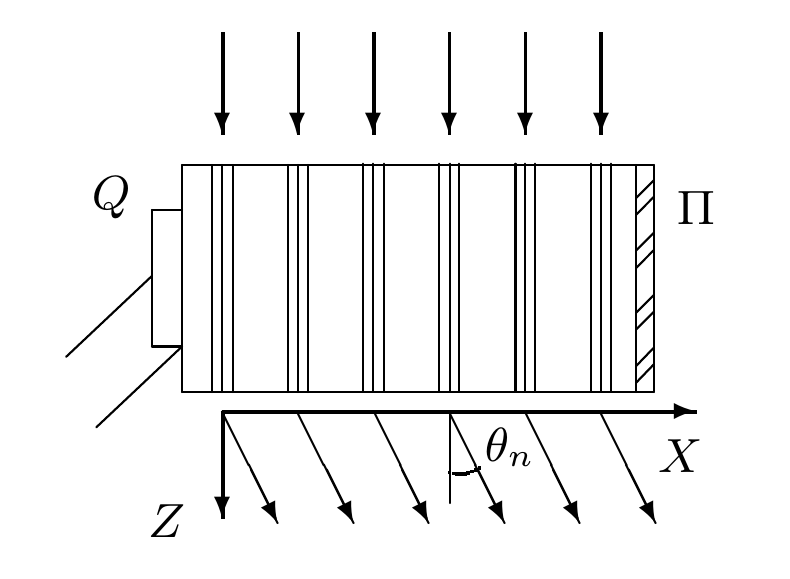
\includegraphics[width=0.4\textwidth]{res/image_1}
		\caption{Дифракция световых волн на акустической решетке}
		\label{diff}
	\end{figure}
	
	Зная положение дифракционных максимумов, легко определить длину ультразвуковой волны, учитывая малость $ \theta $: $ \sin \theta \approx \theta \approx l_m /F  $, где $ l_m $ --- расстояние от нулевого до последнего видимого максимума, $ F $ --- фокусное расстояние линзы. Тогда получим:
	
	\begin{equation*}
		\Lambda = m \lambda F/ l_m 
	\end{equation*}
	Скорость ультразвуковых волн в жидкости, где $ \nu $ --- частота колебаний излучателя:
	
	\begin{equation*}
		v = \Lambda \nu 
	\end{equation*}
	
	\section*{Экспериментальная установка}
	
	Схема установки приведена на рисунке 2. Источник света Л через светофильтр Ф и конденсор К освещает вертикальную щель $ S $, находящуюся в фокусе объектива $ O_1 $. После объектива параллельный световой пучок проходит через кювету С перпендикулярно акустической решетке, и дифракционная картина собирается в фокальной плоскости объектива $ O_2 $ , наблюдается при помощи микроскопа $M$.
	
	Предварительную настройку установки произведем в соответствии с инструкцией с зеленым фильтром, далее в работе используется красный.
	
	\begin{figure}[h!]
		\centering	
		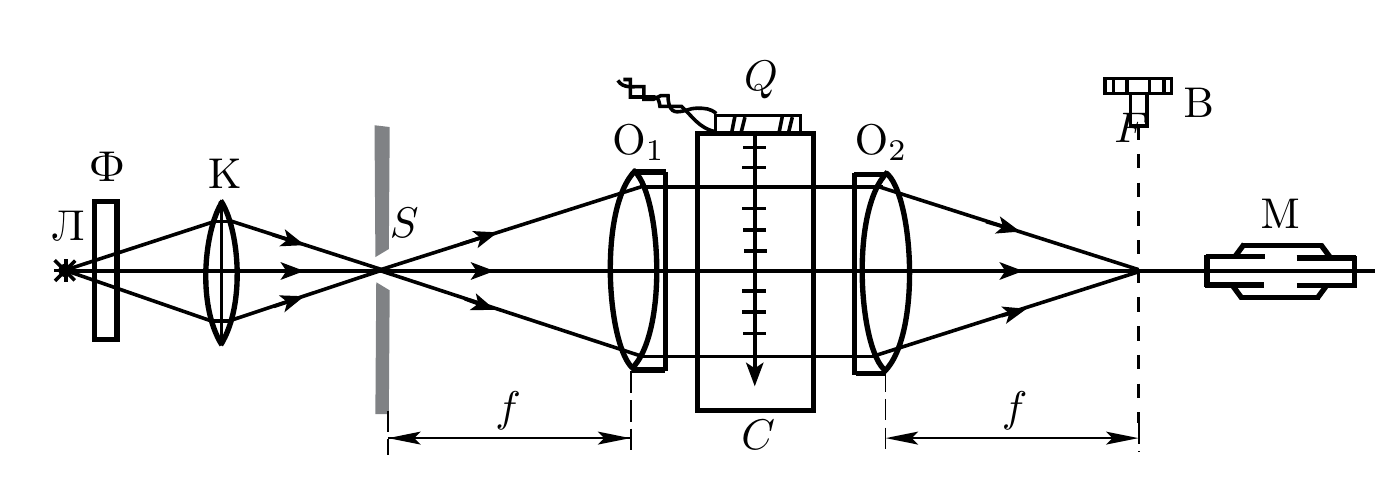
\includegraphics[width=10cm]{res/image_2}
		\caption{Схема для наблюдения дифракции на акустической решетке}
		\label{shema1}
	\end{figure}
	
	Фокусное расстояние объектива $ O_2$: $F = 30 $ см, цена деления винта микроскопа -- 4 мкм, погрешность измерений примем равной  $ \sigma = $ 1 деление, или 4 мкм. Полоса пропускания фильтра $ \lambda = 6400 \pm 200$ \AA.
	
    \section*{Ход работы}
	
	\begin{center}
		\textbf{I. Определение скорости ультразвука по дифракционной картине}
	\end{center}

	\begin{enumerate}
		\item Соберем схему согласно рисунку. Отцентрируем систему и установим ширину щели равной 25 мкм.
		
		\item Получим дифракционную картину.
		
		Перемещая излучатель с помощью лимба, оценим по порядку величины длину УЗ волны как удвоенное расстояние между наиболее четкими картинами: $\Lambda = 2 \cdot 43 \text{ дел}\cdot 10\frac{\text{мкм}}{\text{дел}} = 0.86$ мм.
        Т. к. измерения проведены при $\nu = 1.81$ МГц, то скорость звука $c=\Lambda \nu=1560$ $\frac{\text{м}}{\text{с}}$.
		
		\item Определим положения дифракционных полос. С помощью перекрестия и микрометрического винта, установленного на выходе прибора, определим координату $X$ каждой светлой полосы в делениях винта. 
		
		Проделаем данную операцию для четырех частот. Результаты занесем в таблицу 1.
		Результаты заносим в таблицу 1:
  
        \begin{table}[h!]
    	   \centering
    	   \footnotesize
    	   \begin{tabular}{cc|cc|cc|cc}
\toprule
$m$ & $x_m$, дел & $m$ & $x_m$, дел  & $m$ & $x_m$, дел  & $m$ & $x_m$, дел  \\
\multicolumn{2}{c}{$\nu$ = 1.192 МГц} & \multicolumn{2}{c}{$\nu$ = 1.526 МГц} & \multicolumn{2}{c}{$\nu$ = 1.811 МГц} &\multicolumn{2}{c}{$\nu$ = 3.467 МГц}\\
\midrule
   &     & -3 &	-153& -3 & -184  &    &      \\
-2 & -77 & -2 & -98 & -2 & -115	 & 	  &      \\
-1 & -36 & -1 & -46 & -1 &  -55	 & -1 & -101 \\
 0 &   0 &  0 &   0 &  0 &    0	 &  0 &    0 \\
 1 &  37 &  1 &  48 &  1 &   57	 &  1 &  102 \\
 2 &  79 &  2 & 100 &  2 &  116	 & 	  &      \\
   &     &  3 & 155 &  3 &  185  &    &      \\
\bottomrule
\end{tabular}
    	   \caption{Зависимость $X(m)$ для 4 частот}
    	   \label{tab:t1}
        \end{table}	

  
		\item Построим на одном графике 1 $X = X(m)$ для каждой частоты.

		\begin{figure}[H]
			\centering
			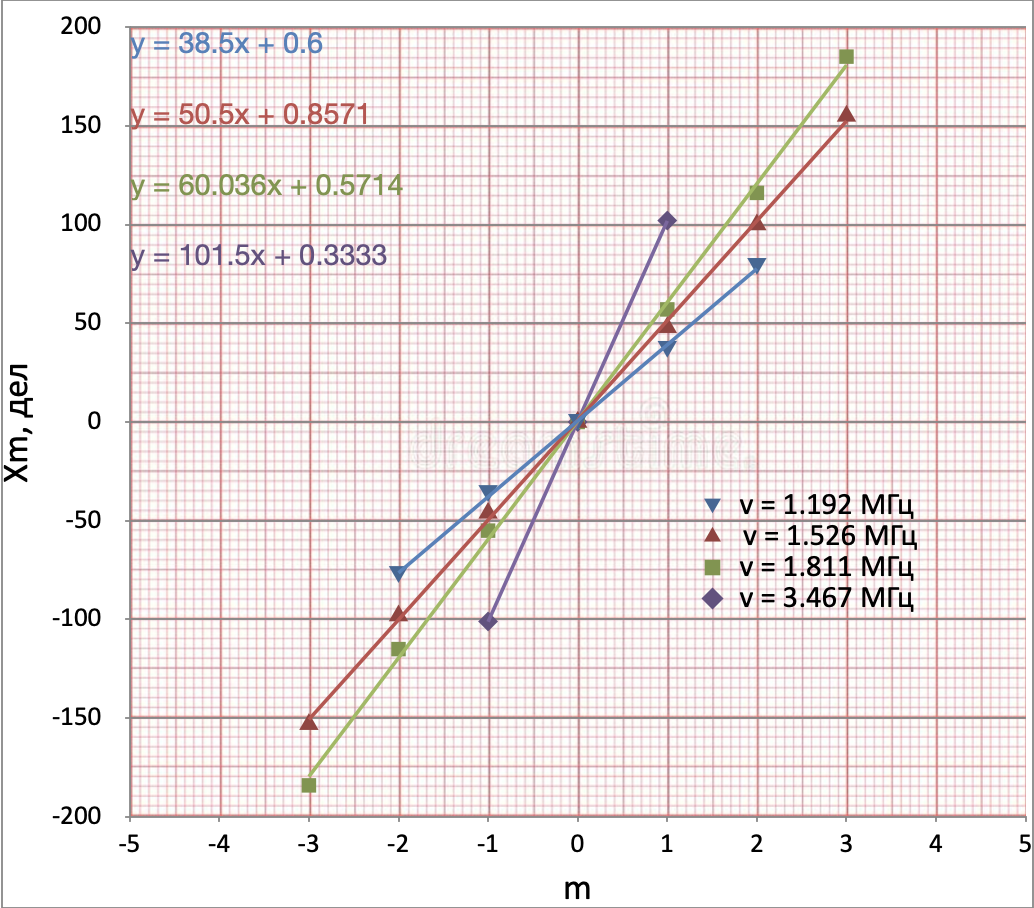
\includegraphics[width=0.8\linewidth]{src/Xm.png}
			\caption{Зависимость $X(m)$ для разных частот}
		\end{figure}

        \item Рассчитаем длину УЗ-волны и скорость звука для каждой частоты.
        \begin{equation}
            \Lambda = \frac{mf\lambda}{X_m} \hspace{30mm} v = \Lambda\nu
        \end{equation}

        \begin{figure}[H]
            \centering
            \footnotesize
            \begin{tabular}{ccc}
\toprule
$\nu$, МГц & $k$, дел & $c$, $\frac{\text{м}}{\text{с}}$ \\
\midrule
1.19 & 38.50	&486.130  \\
1.53 & 50.50	&1450.455 \\
1.81 & 60.04	&1447.938 \\
3.47 & 101.50	&1639.567 \\
\bottomrule
\end{tabular}

            \caption{Зависимость $c$ от $\nu$}
            \label{tab:t2}
        \end{figure}
    
    	Как видно, результаты достаточно близки друг к другу и почти совпадают с табличными значениями: $v = 1500$ м/с.
		
	\end{enumerate}

\newpage
\textbf{II. Определение скорости ультразвука методом темного поля}
	\end{center}

	\begin{enumerate}
		\item Для перехода к методу темного поля отодвинем микроскоп от щели и разместим в промежутке между ними дополнительную линзу.
		
		Поднимем излучатель над кюветой и опустим в воду квадратную сетку. Отцентрируем систему, чтобы сетку было четко видно в микроскопе. Рассчитаем цену деления в этом эксперименте, зная, что размер квадратика сетки 1 мм. Получаем $\boxed{0.14 \frac{\text{мм}}{\text{дел}}}$
		
		
		\item Установим ширину щели 25 мкм. Уберем калибровочную сетки и опустим излучатель. Постараемся увидеть звуковую решетку.
		
		\item Закроем нулевой дифракционный максимум проволочкой. Поле зрения микроскопа затемняется.
		
		\item Меняя частоту, будем наблюдать акустическую решетку.
		
		\item Зафиксируем с помощью окулярной шкалы микроскопа координаты первой и последней из хорошо видимых темных полос и количество светлых промежутков между ними. Проделаем это для 4 разных частот. Результаты пишем в таблицу 3.
		
		\begin{table}[h!]
			\centering
			\begin{tabular}{|c|c|c|c|}
				\hline
				$\nu$, МГц & \begin{tabular}[c]{@{}c@{}}Координата\\ верхней полосы\end{tabular} & \begin{tabular}[c]{@{}c@{}}Координата\\ нижней полосы\end{tabular} & \begin{tabular}[c]{@{}c@{}}Количество\\ светлых полос\end{tabular} \\ \hline
				1.006     & 60                                                                  & 0.0                                                                 & 12                                                                 \\ \hline
				1.190     & 68                                                                  & 0.0                                                                & 20                                                                 \\ \hline
				1.370     & 53                                                                  & 0.1                                                                & 14                                                                 \\ \hline
				1.650     & 67                                                                  & 0.0                                                                 & 20                                                                 \\ \hline
			\end{tabular}
			\caption{Результаты}
		\end{table}
		
		
		\item Для каждой частоты рассчитаем длину $\Lambda$ УЗ-волны.
		Посчитанные значения заносим в таблицу 4.
		\begin{table}[h!]
			\centering
			\begin{tabular}{|c|c|}
				\hline
				$\nu$, МГц & $\Lambda$, мм \\ \hline
				1.0056     & 1.412         \\ \hline
				1.1900     & 1.190         \\ \hline
				1.3700     & 1.060         \\ \hline
				1.6500     & 0.938         \\ \hline
			\end{tabular}
			\caption{Зависимость длины волны от частоты}
		\end{table}
		
		\newpage		
		
		\item Построим график зависимости $\Lambda (1/\nu)$.
		
		\begin{figure}[h!]
			\centering
			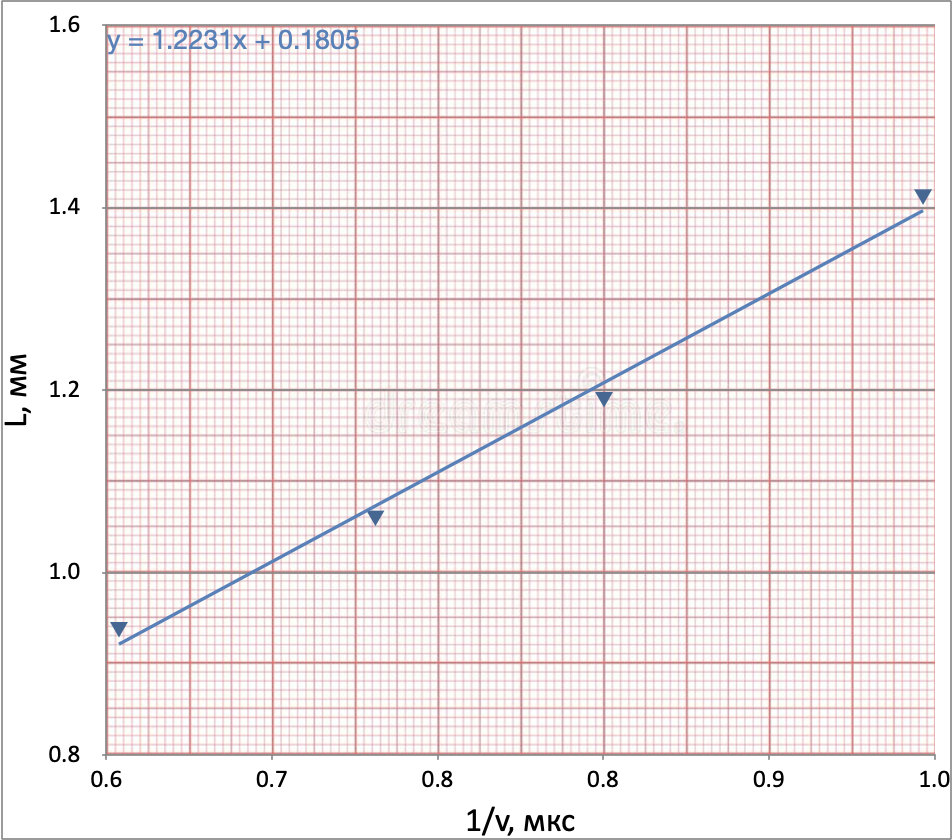
\includegraphics[width=0.8\linewidth]{res/Lambda(nu)}
			\caption{График зависимости $\Lambda (1/\nu)$}
		\end{figure}
		
		По наклону определим скорость ультразвука.
		\begin{equation*}
			v = \Lambda \nu = k = (1.46 \pm 0.09) \; \text{мм} \cdot \text{МГц} = (1460 \pm 90 \; \text{м/с}).
		\end{equation*}
	
		Значение близко к тому, что было найдено ранее. Вдобавок в пределах погрешностей оно совпадает с табличным.
	\end{enumerate}

	\vfill
	\section*{Вывод}
	В данной работе мы изучили дифракцию света на синусоидальной акустической решетке и пронаблюдали фазовую решетку методом темного поля. Помимо этого было определено значение скорости ультразвука в воде: $(1460 \pm 90)$ м/с, что достаточно близко к табличному значению в 1500 м/с и в пределах погрешности вовсе совпадает. Присутствуют ошибки как систематические, так и случайные. Больший вклад вносят последние. Однако общая ошибка составляет не более 9$\%$, что является хорошим результатом. Все эти ошибки связаны с несовершенством техники измерения.
	














\newpage
\begin{thebibliography}{9}
	\bibitem{Siv} Сивухин Д. В. \emph{Общий курс физики. Том 4 Оптика}, 2004
	\bibitem{kirich} Кириченко Н.А. \emph{Оптика.}, 2011
	\bibitem{max} \emph{Лабораторный практикум по общей физике. В 3 томах. Том 3. Оптика: учебное пособие} под ред. А. В. Максимычева, М. Г. Никулина
\end{thebibliography}

\end{document}
